\chapter{Rechnen mit Vektoren}
\begin{inhalt}
  \begin{itemize}
    \item Rechengesetze und Operationen
  \end{itemize}
\end{inhalt}

\section{Grundlagen}
Ein Vektor ist eine mathematische Größe, die durch einen Pfeil dargestellt wird.

\begin{bla}{Der Ortsvektor}
   \begin{marginfigure}[5em]
    \begin{tcolorbox}[colback=white!95!black,colframe=white!75!black,title=CAS:,arc=0mm]
      \begin{scriptsize}
        \textbf{Calculator}: \\*
          - \textsc{Ctrl} + \textsc{(} \( \leadsto \) \( [ \ ] \) \\*
          - erste Zahl eintragen \\*
          - \keys{\return} drücken \( \to \) nächste Zahl
      \end{scriptsize}
    \end{tcolorbox}
  \end{marginfigure}
  In drei Dimensionen schreibt man einen Punkt als Abstand zum Ursprung: $P = (1|2|3)$ bedeutet: Vom Ursprung aus liegt der Punkt eine Einheit in $x$- Richtung, zwei in $y$- und drei in $z$-Richtung.
  \\
  Genauso kann man einen Punkt natürlich auch beschreiben, indem man den Vektor vom Ursprung zu dem Punkt schreibt.
  Das geht genau gleich, nur schreibt man die Zahlen (oder Koeffizienten) jetzt übereinander:
  $\vec{P} = \begin{pmatrix} 1\\2\\3 \end{pmatrix}$
  Wieder bedeuten die Koeffizienten das gleiche:
  "`Gehe vom Ursprung eine Längeneinheit in x-Richtung"' und so weiter.
\end{bla}

\begin{bla}{Rechengesetze}
  %
  \begin{marginfigure}[10em]
    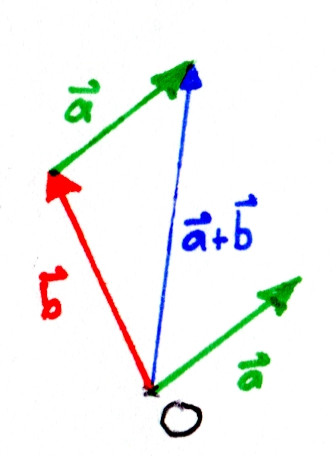
\includegraphics[scale=0.8]{LAGrundlagen1Rechengesetze}
    \caption{Summe zweier Vektoren}
  \end{marginfigure}
  %
  Bei Multiplikation mit dem Faktor $r$ wird der Pfeil einfach länger oder kürzer.
  Bei Addition von zwei Vektoren ergibt sich der Pfeil durchs Hintereinanderzeichnen der zwei Anfangspfeile.
  \begin{enumerate}
    \item $\vec{a} + \vec{b} = \vec{b} + \vec{a} = \begin{pmatrix}
      a_1 + b_1 \\ a_2 + b_2 \\ a_3 + b_3
    \end{pmatrix}$
    \item $r * \vec{a} =
    \begin{pmatrix}
      r * a_1 \\ r* a_2 \\ r * a_3
    \end{pmatrix}$
    \item $r * (\vec{a} + \vec{b}) = r*\vec{a} + r*\vec{b}$
  \end{enumerate}
\end{bla}

\begin{bla}{Strecken und Längen}
  %
  \begin{marginfigure}[10em]
    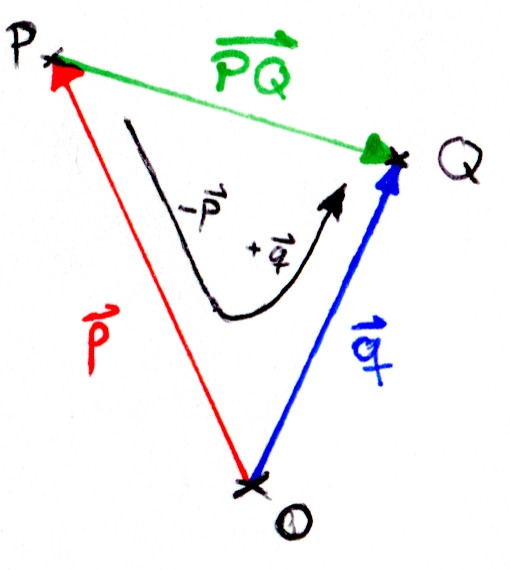
\includegraphics[scale=0.6]{LAGrundlagen2Strecken}
    \caption{Strecke von $P$ nach $Q$}
  \end{marginfigure}
  %
  Die Strecke zwischen zwei Punkten $\overrightarrow{PQ}$ bekommt man, indem man erst von $P$ rückwärts zum Ursprung geht ($-\vec{p}$) und dann (mit $\vec{q}$) vom Ursprung zu $Q$:
  \begin{equation*}
    \overrightarrow{PQ} = - \vec{p} + \vec{q} = \begin{pmatrix}
      q_1\\q_2\\q_3
    \end{pmatrix}
    -
    \begin{pmatrix}
      p_1\\p_2\\p_3
    \end{pmatrix}
    =
    \begin{pmatrix}
      q_1 - p_1 \\ q_2 - p_2 \\ q_3 - p_3
    \end{pmatrix}
  \end{equation*}

  Der Betrag einer Stecke oder die Länge eines Vektors ergeben sich ähnlich zum Satz des Pythagoras:
  \begin{equation*}
    |\overrightarrow{PQ}| = \sqrt{(q_1 - p_1)^2 + (q_2 - p_2)^2 + (q_3 - p_3)^2}
  \end{equation*}
   \begin{marginfigure}
    \begin{tcolorbox}[colback=white!95!black,colframe=white!75!black,title=CAS:,arc=0mm]
      \begin{scriptsize}
        \textbf{Calculator}: \\*
        \menu{Menü > Mat. und Vek > Normen > Norm}
        \( \leadsto \) \textsc{norm}\( \left( \left[ \begin{smallmatrix}
          0 \\ 0 \\ 1
        \end{smallmatrix} \right] \right) \leadsto 1 \)
      \end{scriptsize}
    \end{tcolorbox}
  \end{marginfigure}
\end{bla}

\section{Produkte}
Das Multiplizieren von Vektoren ist ein bisschen komplizierter als bei normalen Zahlen, durch Vektoren zu Teilen ist sogar gar nicht möglich.

\begin{bla}{Skalarprodukt}
   \begin{marginfigure}[5em]
    \begin{tcolorbox}[colback=white!95!black,colframe=white!75!black,title=CAS:,arc=0mm]
      \begin{scriptsize}
        \textbf{Calculator}: \\*
        \menu{Menü > Mat. und Vek > Vek. > SKP} \\*
        \( \leadsto \) \textsc{dotP}\( \left( \left[ \begin{smallmatrix}
          1 \\ 1 \\ 1
        \end{smallmatrix} \right], \left[ \begin{smallmatrix}
          1 \\ 1 \\ 1
        \end{smallmatrix} \right] \right) \leadsto 3 \)
      \end{scriptsize}
    \end{tcolorbox}
  \end{marginfigure}
  Eine hilfreiche Methode um Winkel zu bestimmen ist das sogenannte \emph{Skalarprodukt}:
  \begin{equation*}
    \vec{a} * \vec{b} = (a_1*b_1) + (a_2*b_2) + (a_3*b_3) = |\vec{a}|*|\vec{b}|*\cos(\varphi)
  \end{equation*}
  Hier ist $\varphi$ der Winkel zwischen den beiden Vektoren.
  Das Ergebnis des Skalarproduktes ist ein Skalar, also eine Zahl.
  \\
  Eine sinnvolle Anwendung ist die Suche nach rechten Winkeln:\\
  Wegen des Cosinus ist:
  \begin{equation*}
    \vec{a} * \vec{b} = 0
    \Leftrightarrow
    \varphi = 90\degree
  \end{equation*}
\end{bla}

\begin{bla}{Kreuzprodukt}
   \begin{marginfigure}[5em]
    \begin{tcolorbox}[colback=white!95!black,colframe=white!75!black,title=CAS:,arc=0mm]
      \begin{scriptsize}
        \textbf{Calculator}: \\*
        \menu{Menü > Mat. und Vek > Vek. > Kreuzprod} \\*
        \( \leadsto \) \textsc{crossP}\( \left( \left[ \begin{smallmatrix}
          1 \\ 1 \\ 1
        \end{smallmatrix} \right], \left[ \begin{smallmatrix}
          1 \\ 1 \\ 1
        \end{smallmatrix} \right] \right) \leadsto \left[ \begin{smallmatrix}
          0 \\ 0 \\ 0
        \end{smallmatrix} \right] \)
      \end{scriptsize}
    \end{tcolorbox}
  \end{marginfigure}
  \begin{marginfigure}[0em]
    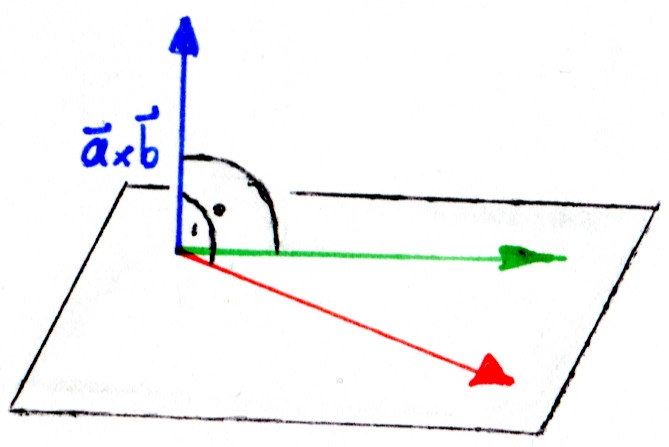
\includegraphics[scale=0.6]{LAGrundlagen3Kreuzprodukt}
    \caption{Kreuzprodukt}
  \end{marginfigure}
Beim \emph{Kreuzprodukt} aus zwei Vektoren ergibt sich ein neuer Vektor:
  \begin{equation*}
      \vec{a} \times \vec{b} =
      \begin{pmatrix}
      a_2 * b_3 - a_3 * b_2 \\
      a_3 * b_1 - a_1 * b_3 \\
      a_1 * b_2 - a_2 * b_1 \\
    \end{pmatrix}
    = - \vec{b} \times \vec{a}
  \end{equation*}
  Dieser neue Vektor steht senkrecht auf den anderen beiden und hat die Länge:
  \begin{equation*}
    |\vec{a} \times \vec{b}| = |\vec{a}| * |\vec{b}| * \sin(\varphi)
  \end{equation*}
\end{bla}

\clearpage

\begin{bla}{Lineare Abhängigkeit}
  Durch Verlängern und Verkürzen eines Vektors $\vec{a}$ kann man eine ganze Gerade erreichen:
  \[
  \text{g: }\ \vec{x} = k * \vec{a}
  \]
  Nimmt man einen zweiten Vektor $\vec{b}$ dazu, gibt es zwei Möglichkeiten:
  %
  \begin{marginfigure}[0em]
    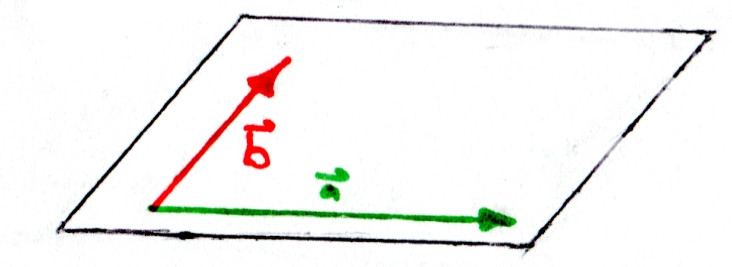
\includegraphics[scale=0.6]{LAGrundlagen4LinAbh1}
    \caption{Zwei linear unabhängige Vektoren spannen eine Ebene auf}
  \end{marginfigure}
  %
  \begin{itemize}
    \item \textbf{$\vec{a}$ und $\vec{b}$ sind parallel:} \\
    Man nennt die beiden \emph{linear abhängig}, weil man immer noch nur die Gerade erreichen kann:
    \[
    \text{g: }\ \vec{x} = k * \vec{a} +  l * \vec{b} =  k * \vec{a}
    \]
    \item \textbf{$\vec{a}$ und $\vec{b}$ laufen in verschiedene Richtungen:} \\
    Man nennt die beiden jetzt \emph{linear unabhängig}, weil man plötzlich eine ganze Ebene erreichen kann:
    \[
    \text{E: }\ \vec{x} = k * \vec{a} +  l * \vec{b}
    \]
  \end{itemize}

  %
  \begin{marginfigure}[-17em]
    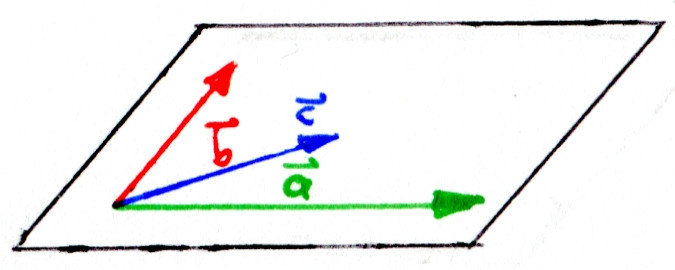
\includegraphics[scale=0.6]{LAGrundlagen4LinAbh2}
    \caption{Drei linear abhängige Vektoren spannen keinen Raum, sondern nur eine Ebene oder Gerade auf}
  \end{marginfigure}
  %
  %
  \begin{marginfigure}
    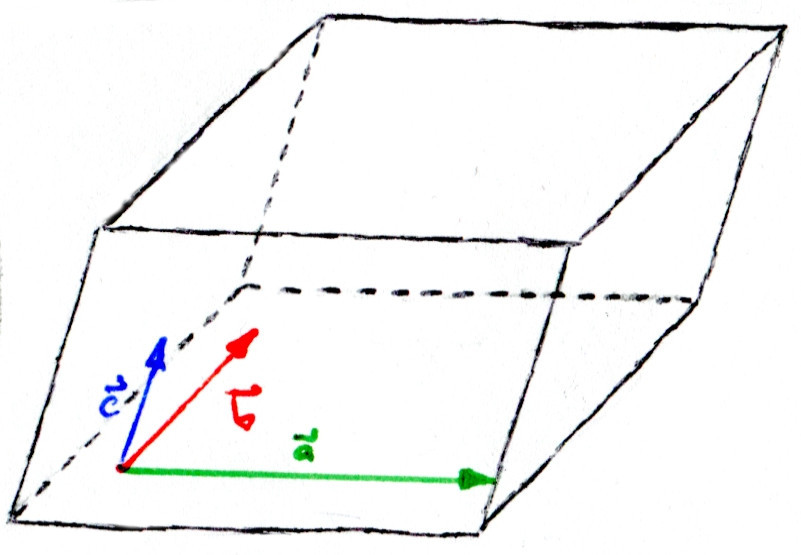
\includegraphics[scale=0.6]{LAGrundlagen4LinAbh3}
    \caption{Drei linear unabhängige Vektoren spannen den gesamten Raum auf}
  \end{marginfigure}
  %
  Als nächstes kann man noch einen dritten Vektor dazunehmen.
  Man nennt die drei dann \emph{linear unabhängig}, wenn man alle Punkte im ganzen Raum erreichen kann und \emph{linear abhängig}, falls man nur eine Ebene oder Gerade erreicht.
\end{bla}
